\chapter{Simplified RL model}
We set up an hybrid Rescorla-Wagner/Pearce-Hall update mechanism following the scheme above.
The V values are updated according to the equation
\begin{equation}
V_s(t+1)=V_s(t)+k\cdot\alpha(t)\cdot\delta  \hspace{0.3cm} with \hspace{0.3cm}\delta(t)=r(t)-V_s(t)
\label{VValues}
\end{equation}
where $\delta$ is the prediction error. Importantly V values are modulated according to the time dependent learning component $\alpha(t)$, this component is directly related to the uncertainty to get the reward. The need to introduce a time dependent learning rate was emphasized first in works as \cite{Daw} and \cite{Funamizu}.
\begin{figure}
    \centering
    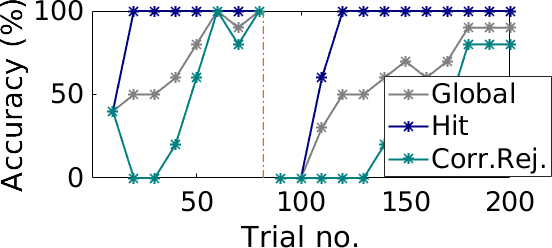
\includegraphics[scale=0.8]{figures/Lastrev1_V05_An6_Perf1.png}
    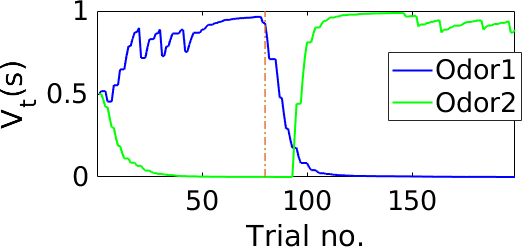
\includegraphics[scale=0.8]{figures/Lastrev1_V05_An6Values.png}
    
    \caption{Caption}
    \label{fig:RL_ex}
\end{figure}

\begin{figure}
    \centering
    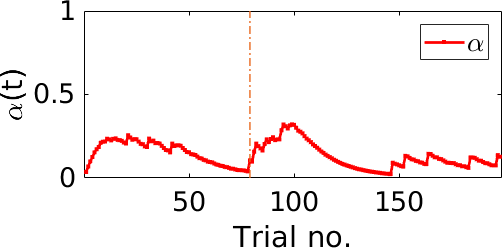
\includegraphics[scale=0.8]{figures/Lastrev1_V05_An6Alpha.png}
    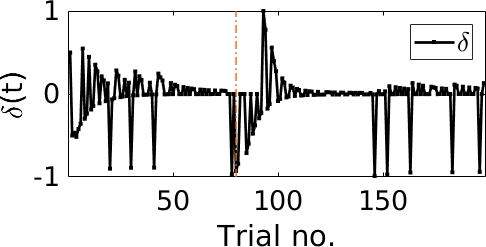
\includegraphics[scale=0.8]{figures/Lastrev1_V05_An6Delta.png}
    \caption{Caption}
    \label{fig:RL_alphadelta}
\end{figure}